\chapter{Methods}
\label{chap:methods}

This chapter goes deeper into the experimental setups used for the experiments, discussed in Chapter \ref{chap:aims}.
All code used for this thesis is available on github (\url{https://github.com/wwelvaer/thesis/tree/main/MassSpecGym}).

\section{Model Training}
\label{sec:training}

All models trained for this thesis use the labeled MassSpecGym dataset, described in Section \ref{subsec:massspecgymdataset}, and follow the de novo model architecture from MassSpecGym~\cite{bushuiev2024massspecgym} closely.
Most of the model architecture code was heavily inspired by MassSpecGym's source code.
It uses the pytorch transformer implementation along with a linear layer before and after the transformer to achieve the requested input and output dimensions for the transformer.
The training algorithm follows the original transformer implementation from \textcite{vaswani2017attention}, using a teacher forcing approach where only ground truth tokens are used to predict the next token at training time.
This results in a model that predicts the probability distribution of the next token given the peaks of a \ac{MS/MS} spectrum along with an already generated context sequence of tokens.
Spectrum peaks are provided as a 2d array with two columns. Each row corresponds to one peak in the spectrum with the value in the first column being its m/z value and the second column its intensity.
The model acts as a classifier for the next token by outputting a vector of length $v$, with $v$ being the number of tokens of the tokenizer.

The exact model used in MassSpecGym suffered from exploding gradients in the first linear layer, which caused the computation to halt by overflow errors.
Several solutions were implemented to combat this problem.

\begin{description}
    \item[Gradient clipping]limits the gradient to [-1, 1],
    when during backpropagation a gradient is not in the interval,
    it is clipped to the closest boundary.
    \item[Lowering learning rate]of the affected layer delays the gradients from overflowing from $3\cdot 10^{-4}$ to $3\cdot 10^{-5}$ and $3\cdot 10^{-6}$.
    \item[Scaling] the m/z values from the peaks in the \ac{MS/MS} spectrum down to the same interval as the intensities from the peaks prevents large differences in the gradients calculation.
    \item[Lowering the floating point precision]by shortening the mantissa to 7 bits instead of 23 bits (see figure~\ref{fig:bf16}), 
    all values get rounded to a lower precision. This rounding acts as a regularization step.
    \begin{figure}[h]
        \centering
        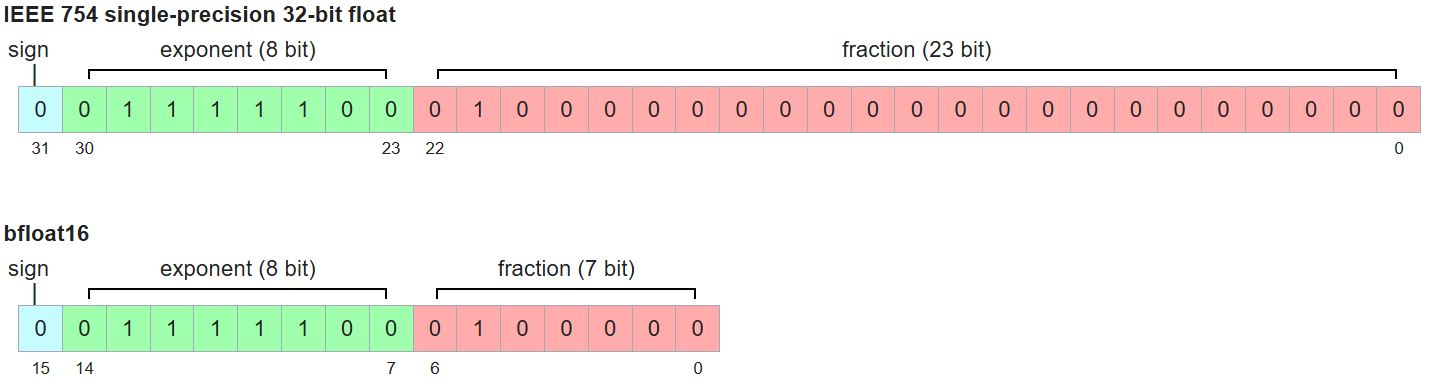
\includegraphics[width=\linewidth]{figures/methods/bf16.JPG}
        \caption{Composition of float32 and bfloat16 (from \url{https://en.wikipedia.org/wiki/Bfloat16_floating-point_format})}
        \label{fig:bf16}
    \end{figure}
    \item[Removing embedding scaling,]because the order of the peaks from the input spectra does not matter,
    no positional encodings are added, there is therefore no need to scale the embedding layer as in the original implementation from \textcite{vaswani2017attention}.
\end{description}

Most of these methods managed to at least delay the problem of exploding gradients, they did however impact the performance significantly compared to the results from MassSpecGym.
Removing the embedding scaling was the only method that fully stabilized training without tanking the performance.
All models described further therefore share the same model architecture as the MassSpecGym de novo models without the embedding scaling step.

Every model was trained using the Adam \cite{kingma2014adam} optimizer with a constant learning rate and an early stopping criterion of five epochs of non-improving validation loss.
All models reached this early-stopping criterion.

All models were trained on the Ugent \ac{HPC} accelgor cluster using a singular NVIDIA Ampere A100 GPU.
Training time without sampling was for every model around 2 hours. 

To replicate the results from MassSpecGym, a hyperparameter gridsearch was conducted for the SMILES model, taking the optimal hyperparameters (with the lowest validation loss) from MassSpecGym's de novo SMILES model results into account
while also extending the search space further than the previously found optimal values.

\section{Samplers}
\label{sec:samplers}

The MassSpecGym paper~\cite{bushuiev2024massspecgym} implemented a simple naive sampling algorithm that iteratively samples from the (with temperature scaled) output distribution of the model, described as the naive approach in Section \ref{sec:samplingmethods}.
This is repeated $n$ times, with $n$ being the prediction amount for each spectrum. The randomness of the sampler results (optimally) in $n$ different predictions.
Because we are interested in a relaxation of the prediction problem, where $n=10$ predictions are evaluated, the sample algorithm was executed 10 times. This was optimized with parallelization.

A big load of the sampling calculation is the forward pass of the transformer model. 
If we work with a GPU that has enough VRAM (at least $n$ times more than would be used for sampling one batch),
we can duplicate the batch $n$ times and feed it through one forward pass of the model. The inherent parallelization of the GPU will then be used more optimally.
An execution time benchmark can be found in Section \ref{sec:sampler_parallelization} of the Appendix.

To benchmark performance of the different sampling algorithms described in Section \ref{sec:samplingmethods}, an implementation was made for each algorithm.
Because the VRAM requirement for the parallelization can be very demanding, two versions of each algorithm were implemented. 
One version uses the parallelization by reducing the number of forward passes (requiring sufficient VRAM on the GPU), the other version repeats the sampling of one batch just like the original MassSpecGym implementation.
These versions will have the same results and will only differ in execution time.

\subsection{Stochastic samplers}
\label{sec:stochastic_samplers}

Stochastic autoregressive sampling algorithms introduce randomness by sampling from the output distribution in a specific manner.
This allows them to be called multiple times to get different predictions from the same spectra as described before.
The simplest stochastic sampling algorithm is the naive method described above.
For this method, the logits from the output of the transformer model were first scaled by a temperature parameter $T$ to shift the output distribution.
After the logits were scaled, a softmax function mapped these to probabilities.
These probabilities were then sampled by the multinomial function from PyTorch.
This was repeated until the maximum prediction length was reached or every prediction in the batch reached the end token.

To reduce randomness and prevent that tokens with small probabilities can be sampled, we can limit the sampling to the top-$k$ tokens with top-$k$ sampling.
Because the tokens with the highest logits will also map to the highest probabilities through the softmax function,
for top-k sampling, we isolated the $k$ tokens with the highest logits before applying the softmax function.
The output probabilities were then calculated for only these $k$ isolated tokens by applying the softmax function to only these logits, which were then sampled with the multinomial function.

Another way to reduce randomness and prevent tokens with low probabilities to be sampled without explicitly declaring the number of tokens $k$ that should be considered is by adding a cumulative probability threshold $p$ with top-p/nucleus sampling.
For this method, The logits were first passed trough the softmax function to get their probabilities.
The tokens were then sorted by their probabilities in a descending order.
From these sorted probabilities, a cumulative distribution was calculated.
The first $m$ tokens for which their cumulative probability just exceeds the threshold $p$ were then selected.
This resulted in the smallest subset of tokens with a cumulative probability exceeding $p$.
These $m$ tokens were then isolated and their probabilities rescaled through the softmax function before being sampled with the multinomial function.

\subsection{Deterministic samplers}

Because there is no randomness in deterministic samplers, the sampling algorithm was not repeated to get $n$ different predictions.
The parallelization optimization was hence not applicable here and only one version of these samplers was implemented.

A greedy approach to remove randomness is to always sample the token with the highest probability.
Because this is the same as the token with the highest logit, no softmax function was needed.
Again, this was repeated until the maximum prediction length was reached or every prediction in the batch reached the end token.
This greedy sampler is only capable of generating one prediction for a spectrum.
Other samplers can become identical to the greedy sampler by choice of parameters, e.g. top-$k$ sampler with $k=1$.

To generate multiple predictions for the same spectrum in a deterministic way, beam search was used.
The scoring function from Section \ref{sec:samplingmethods} was used to score (partial) prediction sequences.
At each time step the beam search algorithm used the transformer model to predict the next token probabilities for each sequence stored in the previous time step.
From these probabilities and their sequence context, new scores are calculated.
The sequences (context + new token) with the highest $b$ scores are then stored for expansion in the next time step.
This is repeated until the maximum prediction length is reached or every $b$ sequences for every spectrum in the batch has reached the end token.
The $n$ predictions with the highest scores are then returned, corresponding to the evaluation setting used.
When $n < b$, predictions will be repeated.

By using a beam width $b=1$, the beam search algorithm was be used as the greedy sampler, no explicit implementation for the greedy sampler was implemented.

\section{BPE as Pretraining}
\label{sec:bpe}

A tokenizer maps a token to a (sequence of) character(s) and back. The set of (sequence of) characters in a tokenizer is called its vocabulary.
All tokenizers in this thesis for which the vocabulary was computed with \acf{BPE}, used the ByteLevelBPETokenizer implementation from huggingface's tokenizers library (\url{https://github.com/huggingface/tokenizers/blob/main/bindings/python/py_src/tokenizers/implementations/byte_level_bpe.py}).
The \ac{BPE} algorithm combines a frequently occurring pair of characters by replacing them with a novel character and storing this replacement in a lookup table.
This novel character can then also be combined further with other characters. 
This is repeated until either the lookup table has reached the desired vocabulary size or there are no more frequently occurring pair of characters in the modified dataset.
These replacements from the lookup table can then be reconstructed to their original character sequences, which represent frequently occurring patterns in the dataset and are stored in the tokenizer's vocabulary.
Because of the replacements in the dataset, these sequences can very in length.

Two important parameters can be set in this algorithm:
(1) The vocab size discussed before. This dictates the maximum number of sequences that can be stored in the vocabulary and will thus decide if the algorithm will be halted early. The default value is 30,000.
(2) The minimum frequency a pair of characters has to occur in the dataset to be stored. The default value is 2.

The unlabeled molecule datasets used to compute the vocabulary from the different tokenizers in this Thesis are from MassSpecGym, see Section \ref{subsec:massspecgymdataset}.
Each \ac{BPE} tokenizer also used the unique training labels from the training set.
The SMILES de novo model from the MassSpecGym paper \cite{bushuiev2024massspecgym} used the dataset with 4,000,000 unlabeled SMILES to precompute a tokenizer vocabulary using \ac{BPE}.
The SELFIES de novo model from the paper did not use \ac{BPE}, the vocabulary of its tokenizer only contains sequences of a single SELFIES tokens.

\section{Augmentation}
\label{sec:augmentation}

All datasets were augmented offline, before training, to preserve execution time on the \ac{HPC} of Ghent University.
Code for the data augmentation can be found as a notebook at \url{https://github.com/wwelvaer/thesis/blob/main/notebooks/augmentation.ipynb}.
For all augmented training sets, a SMILES transformer model was trained with the same hyperparameters from the MassSpecGym paper \cite{bushuiev2024massspecgym}.

\subsection{SMILES augmentation}

SMILES are a one-dimensional representation of a 2d molecular graph.
The traversal algorithm to convert a molecular graph to a SMILES is deterministic.
The same molecular graph will always be converted to the same canonicalized SMILES.
We can randomize this traversal algorithm to create different SMILES for the same molecular graph.
The SMILES are then synonyms of each other, as they represent the same molecule.
RDkit has already implemented the randomized traversal in their MolToSmiles function (\url{https://www.rdkit.org/docs/source/rdkit.Chem.rdmolfiles.html#rdkit.Chem.rdmolfiles.MolToSmiles}).

To generate a SMILES synonym, the original SMILES must be converted to its molecular graph. 
By using the randomized traversal from that graph back to a SMILES we get a synonym.
We can now augment the training dataset by copying the spectrum of a training sample but changing the SMILES label to a random synonym.

Three different augmented training sets were created. One where the training data is duplicated once, twice and five times with SMILES synonyms.
The original training samples with the original SMILES are kept in the datasets.

\subsection{Spectral augmentation}

The \ac{MS/MS} spectra of two identical molecules can be shifted because of different precursor masses.
We can mimic this to augment the training spectra.
Following the methods of DreaMS \cite{bushuiev2024emergence}, all augmented spectra are randomly shifted by applying the same random shift with a maximum m/z range of 50 to all the peaks.
The SMILES labels from the augmented spectra are copied.

Two different augmented training sets were created:
One mimicking DreaMS where $20\%$ of the training spectra are augmented, and one where all training spectra are augmented.
Again, the original training data is kept in the augmented training sets.

\section{Molecular representations}
\label{sec:representations}

All molecular representations used for training different models were translated from the SMILES in the MassSpecGym dataset.
For translation, RDkit was used except for DeepSMILES and SELFIES as these molecular representations have their own packages with the same name.
To ease the implementation of models predicting different molecular representations than SMILES,
we added a translation step before the model input and after the model output.
Hence, all model evaluation metrics were computed on predictions translated back to SMILES.
The translation occurs thus at training and evaluation time.
This method is also used for the de novo SELFIES model in the MassSpecGym paper (see Section \ref{subsec:massspecgymmodels}).
The tokenizer is used to handle translation. Before every encoding, and after every decoding step, a translation step from and to SMILES is performed.
The code used for all tokenizers can be found at \url{https://github.com/wwelvaer/thesis/blob/main/MassSpecGym/mol_tokenizers.py}.

Because SMILES can be rewritten during translation to and from another molecular representation,
the training SMILES are passed through each representation's tokenizer to compute possible translation modifications.
The resulting (possibly modified) training SMILES are then stored for each representation.
When the model predicts a molecule from its training set, the translated SMILES-string will be present in this stored dataset.
This way the amount of de novo predictions can be accurately measured with different molecular representations.

Multiple models were trained on the following molecular representations: SMILES, DeepSMILES, SELFIES and InchI.
For each of the four representations a model was trained using a tokenizer pre-computed with \ac{BPE} on the unlabeled 4 million molecules dataset from MassSpecGym,
mimicking the implementation from the de novo SMILES model. All models used the hyperparameters from this model.
For these representations, a model was also trained using a tokenizer without \ac{BPE}.

To respect the more complex composition of InchI, a model with multiple decoders was created to predict the different layers of an InchI string.
Because only the first three layers encode the 2d composition of a molecule, and we are not interested in 3d composition information such as stereochemistry,
the model only predicts these three layers.
Three decoders are used to predict these layers. These decoders share the exact same architecture used by the decoders from the other models.
Each decoder has its own tokenizer. For simplicity, a parent tokenizer handles these three tokenizers and handles the correct merging of the three predictions by the model.
To train the model, the loss of the model is the sum of the losses from the three decoders.